%% architecture.tex  —  Moufida System Architecture Diagrams
%% Compile from docs/submission/:  pdflatex architecture.tex

\documentclass[11pt,a4paper]{article}

\usepackage[margin=2cm]{geometry}
\usepackage{graphicx}
\usepackage[hidelinks]{hyperref}
\usepackage{xcolor}
\usepackage{booktabs}
\usepackage{enumitem}
\usepackage{tcolorbox}
\usepackage{float}
\usepackage{caption}
\usepackage{microtype}
\usepackage{titlesec}
\usepackage{pdflscape}
\tcbuselibrary{skins,breakable}

\graphicspath{{./}}

%% ── Palette ──────────────────────────────────────────────────────────────────
\definecolor{ArchNavy}{RGB}{22,40,80}
\definecolor{ArchSlate}{RGB}{50,65,80}
\definecolor{DescBg}{RGB}{245,247,250}
\definecolor{DescFrame}{RGB}{120,140,165}
\definecolor{Accent}{RGB}{200,70,50}   % used sparingly for emphasis

%% ── Spacing ──────────────────────────────────────────────────────────────────
\setlength{\parskip}{6pt plus 2pt minus 1pt}
\setlength{\parindent}{0pt}
\setlist{itemsep=2pt, topsep=3pt, parsep=0pt, leftmargin=1.4em}

%% ── Section styling ──────────────────────────────────────────────────────────
\titlespacing*{\section}{0pt}{16pt}{6pt}
\titlespacing*{\subsection}{0pt}{12pt}{4pt}
\titleformat{\section}{\large\bfseries\color{ArchNavy}}{{\thesection}}{0.6em}{}%
  [\vspace{-2pt}\color{ArchNavy}\titlerule]
\titleformat{\subsection}{\normalsize\bfseries\color{ArchSlate}}{{\thesubsection}}{0.6em}{}

%% ── Description box ──────────────────────────────────────────────────────────
\newtcolorbox{descbox}{
  colback=DescBg, colframe=DescFrame, boxrule=0.5pt, arc=3pt,
  boxsep=3pt, top=4pt, bottom=4pt, left=6pt, right=6pt,
  coltitle=white, breakable
}

%% ── Custom figure caption style ─────────────────────────────────────────────
\captionsetup[figure]{%
  labelfont={bf,color=ArchNavy}, textfont={color=ArchSlate},
  margin=10pt, font=small, skip=4pt
}

%% ── Title ────────────────────────────────────────────────────────────────────
\title{%
  {\color{ArchNavy}\rule{\linewidth}{1.5pt}}\\[6pt]
  \textbf{\Large Moufida --- System Architecture Diagrams}\\[4pt]
  {\normalsize Component, Database, and Interaction Diagrams}\\[6pt]
  {\color{ArchNavy}\rule{\linewidth}{0.8pt}}
}
\author{Team Makrouna Kadheba}
\date{AINS 2026}

\begin{document}
\maketitle\thispagestyle{empty}

\begin{abstract}\small
  This document presents five architecture diagrams for the Moufida platform:
  a full system component diagram showing the two-layer deployment (host machine and
  Docker Compose stack), a database entity-relationship diagram covering the core business
  and telemetry tables, and three sequence diagrams illustrating the most significant
  runtime flows --- full diagnosis, Go daemon hot-swap on project focus change, and the
  creation mode axis-generation loop.
\end{abstract}

\tableofcontents
\vspace{6pt}
\noindent\color{ArchNavy}\rule{\linewidth}{0.4pt}

%% ─────────────────────────────────────────────────────────────────────────────
\section{System Component Diagram}
%% ─────────────────────────────────────────────────────────────────────────────

\begin{descbox}
  The component diagram shows the full Moufida deployment split into two layers.
  \begin{itemize}
    \item The \textbf{Host Machine} layer runs natively: the Tauri desktop app
          (React + TypeScript + Rust), the Ollama LLM engine serving
          \texttt{llama3.1:8b} and \texttt{bge-m3}, and the voice processing pipeline
          (Whisper for STT, Piper and Kokoro for TTS). These run outside Docker to
          access GPU acceleration and the OS audio subsystem.
    \item The \textbf{Docker Compose} layer contains every backend service: the
          orchestrator (FastAPI + LangGraph), 10 expert axis microservices, the
          Knowledge Retrieval Engine (Qdrant + BM25 + RRF), the Analytics \& Signal
          Processor (Rust, CBM + Axis Probe), the Decision Scoring Engine (Affinitree),
          the Background Event Daemon (Go), and the three data stores
          (PostgreSQL, Redis, Qdrant).
    \item All LLM inference from inside Docker routes through
          \texttt{host.docker.internal:11434} --- no model weights live inside containers.
  \end{itemize}
\end{descbox}

\begin{figure}[htbp]
  \centering
  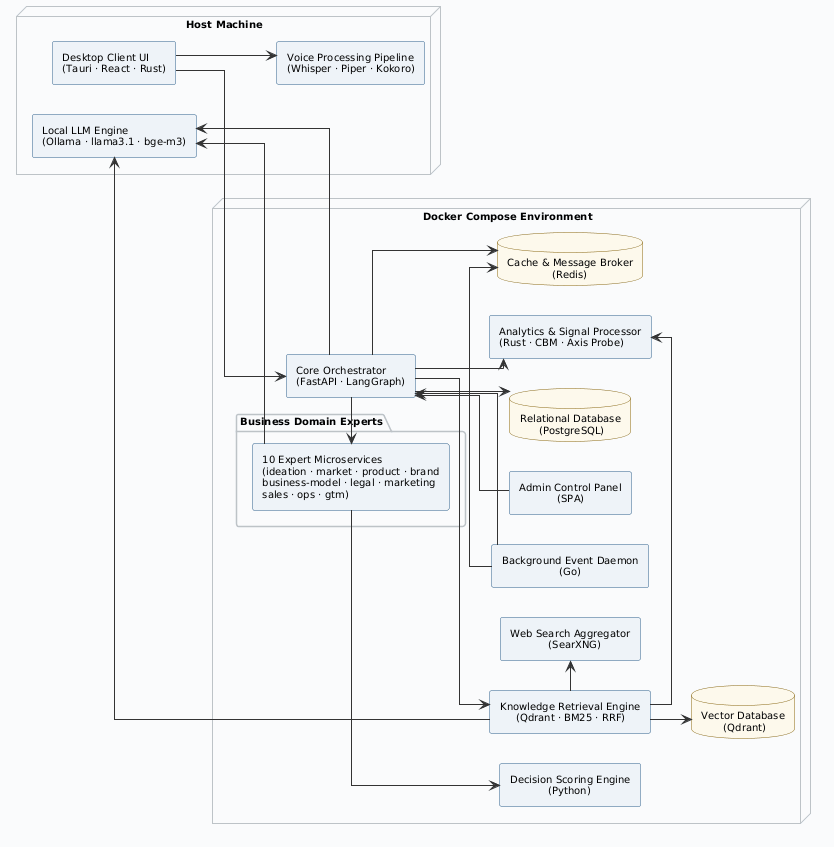
\includegraphics[width=0.9\linewidth,keepaspectratio]{component_diagram.png}
  \caption{Full System Component Diagram}
  \label{fig:component}
\end{figure}

%% ─────────────────────────────────────────────────────────────────────────────
\section{Database Entity-Relationship Diagram}
%% ─────────────────────────────────────────────────────────────────────────────

\begin{descbox}
  The ER diagram covers the core business and telemetry tables. All entities are
  project-scoped through a foreign key to \texttt{profiles}.
  \begin{itemize}
    \item \texttt{profiles} is the root aggregate. Every table references it directly,
          making project deletion straightforward and audit queries project-scoped.
    \item \texttt{score\_snapshots} carries a \texttt{locked} boolean. A locked snapshot
          cannot be overwritten by a subsequent automatic diagnostic, preserving
          human-expert overrides entered via the Score Debate feature.
    \item \texttt{concept\_scores} stores the per-axis CBM output (concept vector,
          CBM score, and identified bottleneck) separately from the main score,
          so the explainability layer can be queried independently.
    \item \texttt{roadmap\_versions} records the \texttt{kb\_version} at generation time,
          enabling stale-roadmap detection when the knowledge base is updated.
  \end{itemize}
\end{descbox}

\begin{landscape}
  \begin{figure}[htbp]
    \centering
    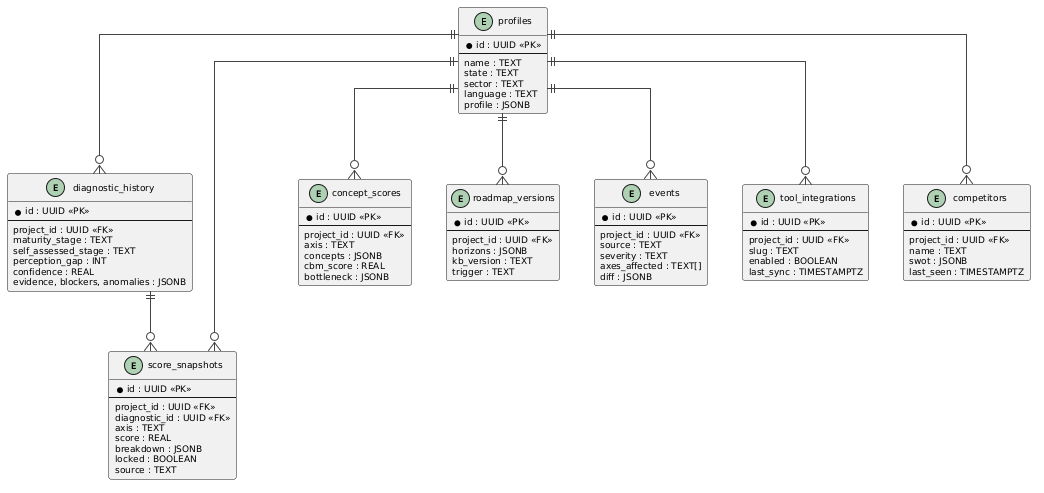
\includegraphics[width=\linewidth,keepaspectratio]{ER_diagram.png}
    \caption{Database Entity-Relationship Diagram (core tables)}
    \label{fig:er}
  \end{figure}
\end{landscape}

%% ─────────────────────────────────────────────────────────────────────────────
\section{Sequence Diagrams}
%% ─────────────────────────────────────────────────────────────────────────────

\subsection{Full Diagnosis Flow}

\begin{descbox}
  This sequence covers the complete diagnostic pipeline from the founder clicking
  ``Diagnose'' to the dashboard updating via SSE.
  \begin{itemize}
    \item Tool integrations run first to upgrade evidence tiers (T1 $\to$ T3) before
          any scoring occurs, so the Affinitree multipliers reflect the best available evidence.
    \item Axis services are dispatched in three dependency-ordered waves using
          \texttt{asyncio.gather} within each wave; each axis independently calls
          Affinitree, RAG, and Ollama.
    \item The CBM pass runs after all wave scores are collected: the orchestrator sends
          concept-scoring prompts to Ollama in parallel, then calls the Signal service
          for bottleneck computation.
    \item Scores, maturity update, and concept update are streamed as SSE events so the
          dashboard renders progressively rather than waiting for the full pipeline.
  \end{itemize}
\end{descbox}

\begin{figure}[htbp]
  \centering
  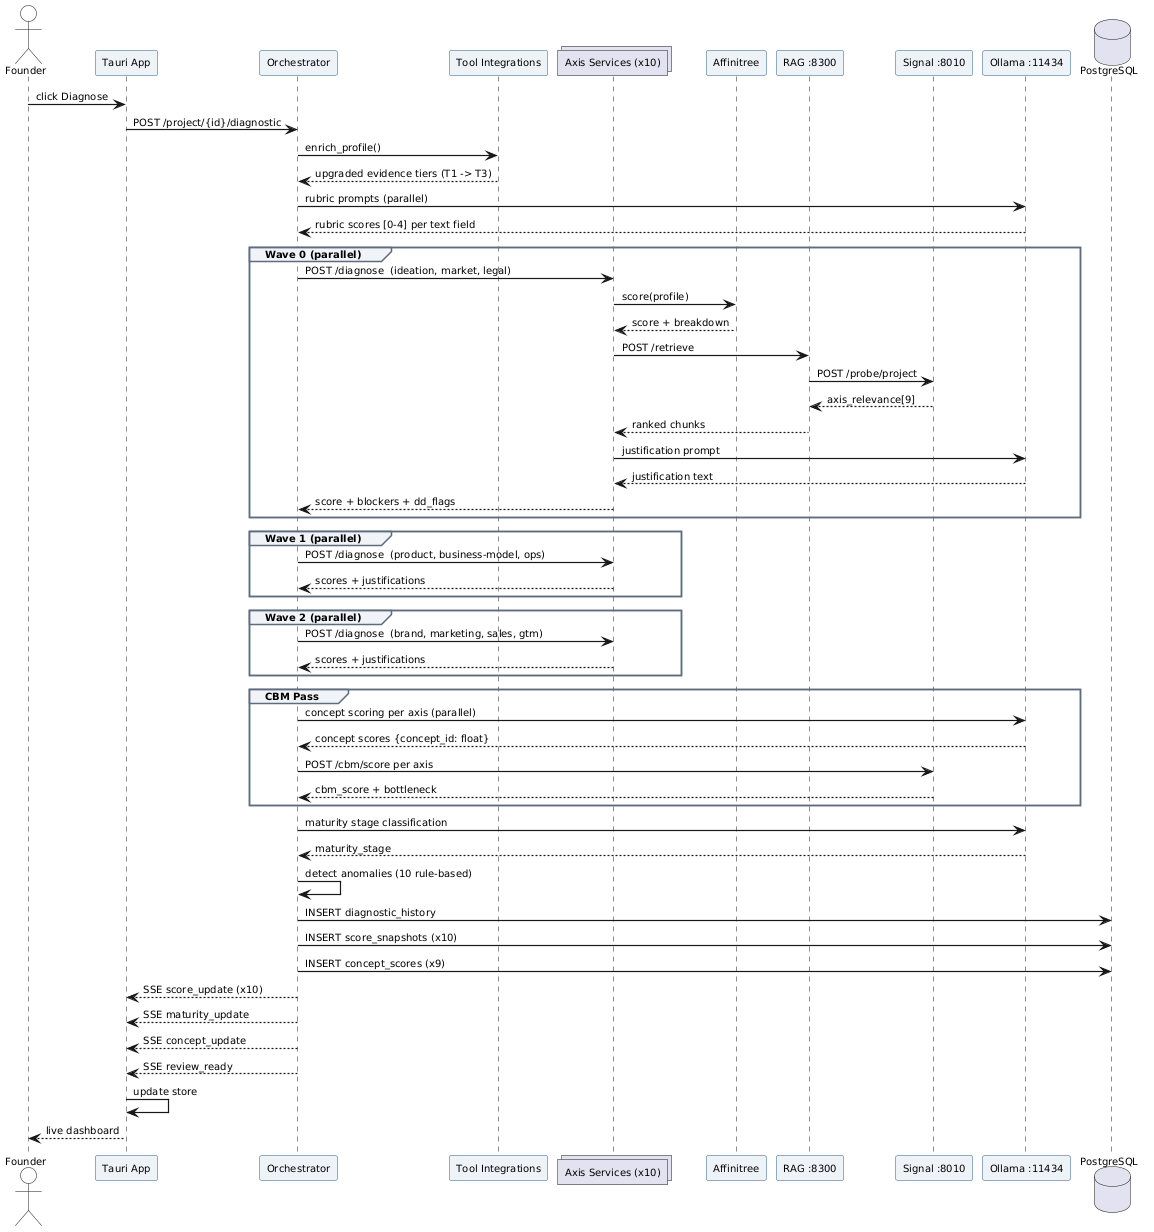
\includegraphics[width=\linewidth,keepaspectratio]{diagnose_seq_diagram.png}
  \caption{Sequence Diagram --- Full Diagnosis Flow}
  \label{fig:seqdiag}
\end{figure}

\subsection{Go Daemon Hot-Swap on Project Focus Change}

\begin{descbox}
  When the founder switches focused project, the daemon tears down its current
  watcher batch and restarts for the new project entirely in-process.
  \begin{itemize}
    \item The daemon polls the orchestrator's heartbeat endpoint every 30 seconds.
          The orchestrator reads \texttt{focus\_project\_id} from the single-row
          \texttt{daemon\_control} table; a changed value triggers hot-swap.
    \item Cancellation uses Go's \texttt{context.CancelFunc}: the supervisor calls
          \texttt{context.Cancel()} and waits on a \texttt{sync.WaitGroup} until
          all goroutines in batch A have drained.
    \item Watch targets (competitor URLs, search keywords, legal feeds) for the new
          project are requested from the orchestrator and cached by profile hash,
          so repeated focus switches to the same project do not re-derive targets.
    \item Six watchers start for the new project: Budget (6 h), Competitor (12 h),
          Legal (24 h), Milestone (24 h), Trend (7 d), Grant (24 h).
  \end{itemize}
\end{descbox}

\begin{landscape}
  \begin{figure}[htbp]
    \centering
    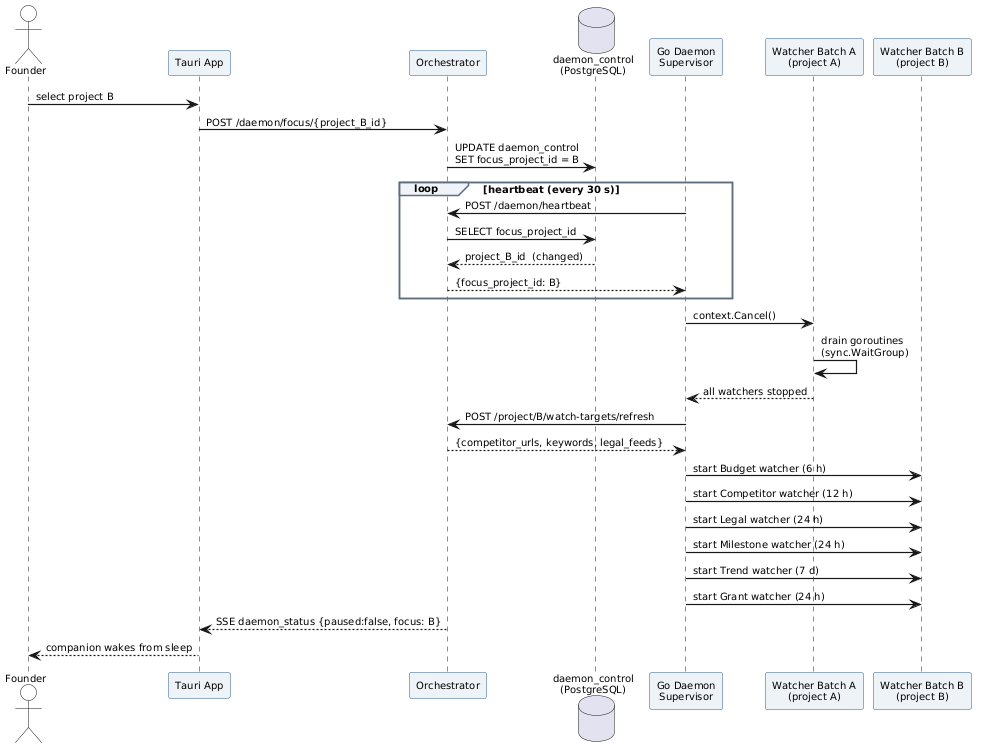
\includegraphics[width=\linewidth,keepaspectratio]{daemon_seq_diagram.png}
    \caption{Sequence Diagram --- Daemon Hot-Swap on Project Focus Change}
    \label{fig:seqdaemon}
  \end{figure}
\end{landscape}

\subsection{Creation Mode --- Axis Generation Loop}

\begin{descbox}
  Creation mode walks the founder through nine axes, one at a time, with an
  approve / edit / retry loop at each step.
  \begin{itemize}
    \item Each generation call fetches fresh KB evidence from RAG and live web results
          from SearXNG so every proposal is grounded in citations, not hallucinated.
    \item The \textbf{Approve} path inserts a \texttt{plan\_sections} row with
          \texttt{approved=true}; older proposals for the same axis are marked
          \texttt{superseded=true}.
    \item The \textbf{Edit with constraints} path replays the generation call with the
          founder's constraints appended to the evidence block, producing a targeted revision.
    \item After all nine axes are approved, \texttt{POST /finalize} triggers roadmap
          generation that synthesises all plan sections into three time horizons with
          full KB provenance recorded in \texttt{roadmap\_versions}.
  \end{itemize}
\end{descbox}

\begin{figure}[htbp]
  \centering
  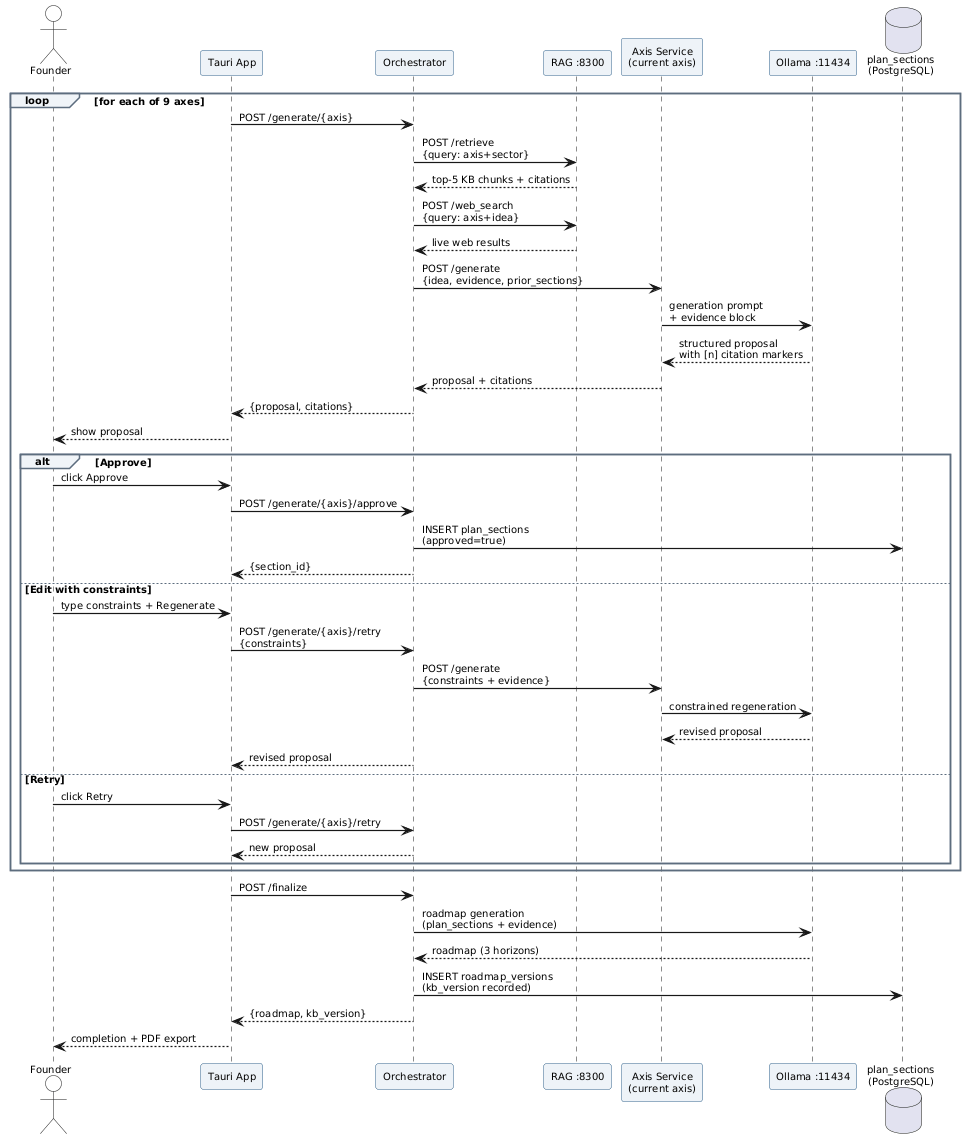
\includegraphics[width=\linewidth,keepaspectratio]{creation_mode_seq_diagram.png}
  \caption{Sequence Diagram --- Creation Mode Axis Generation Loop}
  \label{fig:seqcreation}
\end{figure}

\end{document}